% Progress report for Assoc. Prof. Jesper Rindom Jensen (Aalborg University).
% Build: make report   (or: python report/make_figures.py; cd report; latexmk -pdf jensen_report.tex)
% The figures are drawn by make_figures.py from the committed result CSVs;
% every number in the text is computed from the files listed in Appendix A.
\documentclass[11pt,a4paper]{article}

\usepackage[T1]{fontenc}
\usepackage[utf8]{inputenc}
\usepackage{lmodern}
\usepackage{textcomp}
\usepackage[a4paper,margin=2.5cm]{geometry}
\usepackage{microtype}
\usepackage{graphicx}
\usepackage{booktabs}
\usepackage{tabularx}
\usepackage{array}
\usepackage[font=small,labelfont=bf,labelsep=period,skip=6pt]{caption}
\usepackage{enumitem}
\usepackage{parskip}
\usepackage[section]{placeins}
\usepackage{xcolor}
\usepackage{xurl}
\usepackage{hyperref}

\definecolor{linkblue}{HTML}{1C5CAB}
\hypersetup{colorlinks=true, linkcolor=linkblue, citecolor=linkblue, urlcolor=linkblue,
  pdftitle={Overlapped speech in AMI meetings: diarisation error and speaker attribution},
  pdfauthor={Aaditya Kumawat}}
\DeclareUnicodeCharacter{2212}{\textminus}
% keep each subsection's tables and figures inside it (placeins is strict without [above])
\let\oldsubsection\subsection
\renewcommand{\subsection}{\FloatBarrier\oldsubsection}

\setlist{itemsep=3pt, topsep=3pt, parsep=0pt}
\setlength{\tabcolsep}{5pt}
\newcolumntype{L}{>{\raggedright\arraybackslash}X}
\renewcommand{\arraystretch}{1.12}

\begin{document}

\begin{center}
  {\LARGE\bfseries Overlapped speech in AMI meetings:\\[3pt] diarisation error and speaker attribution\par}
  \vspace{10pt}
  {\large Progress report for Assoc.\ Prof.\ Jesper Rindom Jensen\\ Audio Analysis Lab, Aalborg University\par}
  \vspace{8pt}
  {Aaditya Kumawat \quad\textperiodcentered\quad Indian Institute of Technology Delhi \quad\textperiodcentered\quad 9 November 2026\par}
\end{center}
\vspace{4pt}

\section*{Summary}

Overlapped speech is a quarter of what is said in the 16 AMI test meetings, and it is where diarisation and speaker attribution fail most. I measured how much, under which scoring choices, and why, for pyannote 3.1 and NVIDIA's Sortformer with Whisper. Every comparison below holds in at least 13 of the 16 meetings on each microphone; brackets are 95\% bootstrap intervals over meetings.

\begin{enumerate}[leftmargin=*, label=\arabic*.]
  \item \textbf{Overlap is where diarisation fails.} Against the standard AMI reference, pyannote 3.1 makes 56\% of its DER on the headset mix (52\% on the distant microphone) in overlapped speech, which is 27\% of the scored speaker time. The Forgiving convention reports 6.7\% DER for output that scores 18.8\% under Full.
  \item \textbf{One speaker per word is an error source of its own.} With perfect diarisation, the word-to-speaker rule credits 47\% of overlapped words to the wrong person (43\% with forced-alignment turns).
  \item \textbf{With Whisper, assigning words costs more than diarisation.} pyannote's 33.4\% cpWER on the headset mix splits into 24.2 points of transcription, 7.3 of word assignment and 2.0 of diarisation.
  \item \textbf{Whisper keeps the louder talker.} In overlap it deletes 65\% of a talker's words when they are more than 10~dB below the other talkers, and 34\% when they are more than 10~dB above.
  \item \textbf{The fixed mapping in the plan is lenient, not strict.} Mapping several system speakers to one person forgives pyannote's over-clustering (96 system speakers for 63 people); a fixed one-to-one mapping gives the permutation-invariant score.
  \item \textbf{The reference's word timings decide which diariser wins on DER.} pyannote has 18.8\% and Sortformer 29.4\% against the standard reference; against forced-alignment labels of the same meetings, 36.2\% and 15.9\%.
  \item \textbf{A diariser that follows the louder talker keeps overlapped words with the right person.} Sortformer's cpWER in overlap is 10.4 points [5.7, 13.5] below pyannote's; over all words the two are level.
\end{enumerate}

Findings 2, 4 and 7 point to the next step: recover the quieter talker before recognition, and give words to speakers from acoustic evidence rather than from timestamps.

\section{Aims}

The plan we agreed has two measurements, both on the same systems and meetings.

\begin{itemize}[leftmargin=*]
  \item \textbf{A.\ Overlap-conditioned DER.} Split DER into missed speech, false alarm and speaker confusion, scored separately in single-speaker and overlapped regions, under the scoring conventions in common use (no collar or a 0.25~s collar; overlap scored or excluded).
  \item \textbf{B.\ A speaker-attribution measure without a permutation search.} Map each system speaker to a person once, by majority overlap in single-speaker speech, keep that mapping fixed, and score each word as correctly or wrongly attributed, inside and outside overlap. Compare it with cpWER, the permutation-invariant word error rate.
\end{itemize}

I also tested the two explanations the results suggested: where the attribution errors come from (transcription, the word-to-speaker rule or diarisation), and whose words are lost in overlap.

\section{Data, systems and scoring}

All systems run as published, with nothing tuned on the test meetings, and every scorer is checked against a reference implementation.

\begin{center}
\small
\begin{tabularx}{\textwidth}{@{}>{\raggedright\arraybackslash}p{3.15cm}L@{}}
\toprule
Part & What I used, and how it was checked \\
\midrule
Meetings & AMI full-corpus ASR test set~\cite{ami}: 16 meetings (IS1009a--d, ES2004a--d, TS3003a--d, EN2002a--d), 63 participants; headset mix (IHM-Mix) and single distant microphone (SDM, Array1-01) \\
Diarisation reference & The pyannote AMI setup~\cite{amisetup}, only\_words annotation: speech is the time covered by AMI's manual word times, scored inside the setup's UEMs. Forced-alignment labels of the same words (Horiguchi et al.~\cite{horiguchi}) serve as a second reference \\
Word reference & AMI manual annotations 1.6.2: 88,828 test words with times (89,443 tokens after normalisation); 99.998\% of word midpoints fall inside their speaker's reference turn \\
Second recording & Supreme Court argument in \emph{New York State Rifle \& Pistol Association v.\ City of New York} (2 December 2019)~\cite{oyez}: 62~min, 10 speakers, reference from Oyez's turns and transcript (not hand-corrected, no overlap marked) \\
Diariser 1 & pyannote/speaker-diarization-3.1~\cite{pyannote}: the authors' published AMI test outputs. My own CPU run matches them on the meetings finished so far (14.8\% against 14.7\% DER on three distant-microphone meetings) \\
Diariser 2 & NVIDIA streaming Sortformer v2.1 (NeMo 2.7.3)~\cite{sortformer}, the optional NeMo system in the plan, on CPU with its default post-processing. Against the forced-alignment reference it reproduces its model card's AMI headset-mix DER (15.9\%) \\
Speech recognition & Whisper large-v3-turbo~\cite{whisper} (faster-whisper, int8, beam 5, temperature fallback, voice-activity filter), with Whisper's own word times. Checked with large-v3 on two meetings and with WhisperX forced alignment~\cite{whisperx} on all 16 headset-mix meetings \\
Word to speaker & Each word goes to the system speaker whose turns overlap it most, the rule WhisperX uses \\
DER scorer & My frame scorer at 1~ms with md-eval's optimal one-to-one mapping~\cite{mdeval}; identical to md-eval on 132 real and 980 synthetic comparisons \\
Word scorers & My cpWER, which assigns each error to a region; MeetEval's~\cite{meeteval} diarisation-invariant cpWER (transcription only) and tcpWER (5~s collar). My counts equal MeetEval 0.4.3's on every meeting \\
Text & Whisper's English text normaliser, per word; AMI's letter-spelled acronyms (L\_C\_D) joined \\
Statistics & Rates pooled over meetings; 95\% percentile bootstrap over meetings (10,000 resamples, fixed seed); paired differences; exact sign tests over meetings \\
\bottomrule
\end{tabularx}
\end{center}

Regions come from the reference: a frame is in overlap when two or more reference speakers are active, and a word when its midpoint is. Overlap is 27.0\% of the scored speaker time and holds 24.7\% of the reference words.

\section{Results}

\subsection{Overlap-conditioned DER}\label{sec:der}

Against the standard reference, overlap is 27\% of the scored speaker time but 56\% of pyannote's DER on the headset mix, and the scoring convention alone changes DER by a factor of 2.4 to 2.8 (Tables~\ref{tab:conventions} and~\ref{tab:where}, Figure~\ref{fig:der}).

\begin{figure}[htbp]
\centering
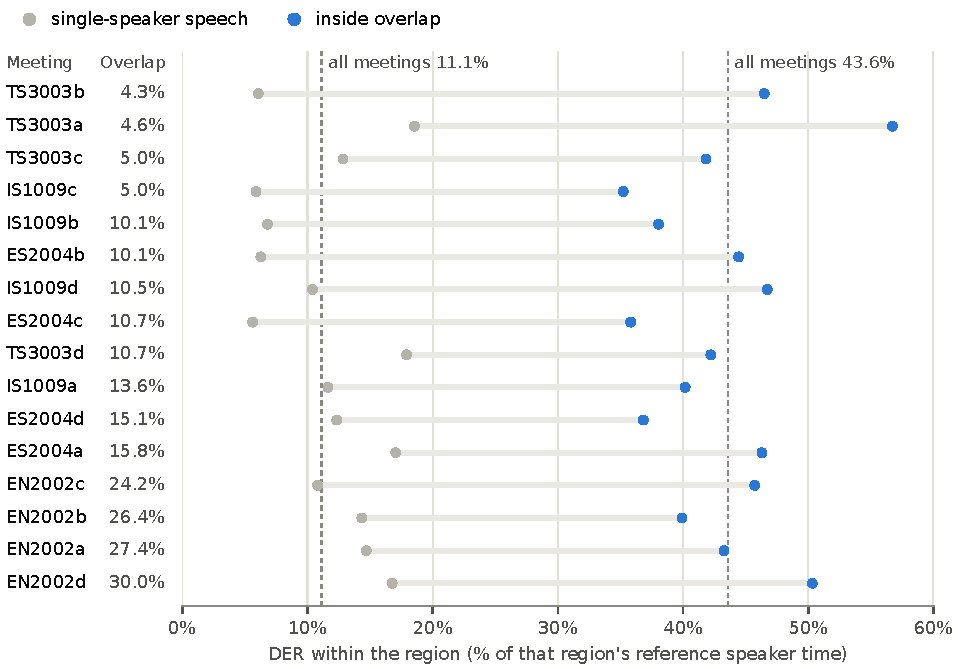
\includegraphics[width=\textwidth]{figures/fig1_der_by_meeting.pdf}
\caption{\textbf{In all 16 meetings, DER inside overlap is 2.4 to 7.7 times DER outside it.} pyannote 3.1, single distant microphone, Full convention. Meetings are sorted by their overlap share (the share of speech time with two or more reference speakers); the dashed lines are the 16 meetings pooled. Source: \texttt{results/decomp\_pyannote31/per\_file.csv}.}
\label{fig:der}
\end{figure}

\begin{table}[htbp]
\centering
\caption{\textbf{The same output under four conventions.} The last row is a paired difference.}
\label{tab:conventions}
\small
\begin{tabular}{@{}lllll@{}}
\toprule
Convention & Collar & Overlap & Headset mix DER & Distant mic DER \\
\midrule
Full & none & scored & 18.80\% [15.69, 21.75] & 22.45\% [18.81, 25.91] \\
Fair & 0.25~s & scored & 12.21\% [8.89, 15.46] & 15.21\% [11.32, 18.97] \\
No collar, overlap excluded & none & excluded & 11.37\% [9.98, 12.95] & 14.62\% [12.57, 16.90] \\
Forgiving & 0.25~s & excluded & 6.66\% [5.59, 7.89] & 9.37\% [7.58, 11.37] \\
\midrule
Hidden by Forgiving & & & 12.14 points [9.50, 14.59] & 13.07 points [10.42, 15.55] \\
\bottomrule
\end{tabular}
\end{table}

\begin{table}[htbp]
\centering
\caption{\textbf{Where the error is} (Full convention).}
\label{tab:where}
\small
\begin{tabular}{@{}lll@{}}
\toprule
 & Headset mix & Distant mic \\
\midrule
Overlap's share of scored speaker time & 27.0\% & 27.0\% \\
Overlap's share of all error & 55.8\% [44.3, 64.0] & 52.5\% [41.5, 60.6] \\
DER inside overlap & 38.9\% [36.1, 40.9] & 43.6\% [40.6, 46.1] \\
\quad of which missed speech / confusion & 25.0\% / 13.9\% & 27.5\% / 16.1\% \\
DER in single-speaker speech & 8.2\% [6.6, 9.8] & 11.1\% [9.0, 13.5] \\
\bottomrule
\end{tabular}
\end{table}

Most of the overlap error is missed speech: pyannote shows one speaker where two are talking. It shows two speakers for 64\% of the overlapped time on the headset mix [59, 67] and 59\% on the distant microphone [54, 62], and 85--86\% of what it marks as overlap is real. Its segmentation model outputs at most two speakers per frame, while 16\% of the overlapped time has three or more people talking.

The 0.25~s collar alone removes half of the overlapped time from scoring (50.4\% kept [40.7, 56.4]), which is why the Fair and Forgiving numbers fall so far. Fixing the speaker mapping on single-speaker frames, as metric B does, changed the mapping in 1 of 32 meeting--microphone pairs and DER by at most 0.006 points: for this system, permutation-invariant and fixed-mapping DER coincide.

\subsection{Who is credited with each word}\label{sec:attr}

With perfect diarisation, the one-speaker-per-word rule credits 47.2\% of overlapped words to the wrong person, and the fixed mapping from the plan forgives errors rather than exposing them (Table~\ref{tab:attr}, Figure~\ref{fig:outcomes}). Here each of the 88,828 true test words, at its true time, goes to a system speaker by the rule, so no speech recognition is involved.

\begin{table}[htbp]
\centering
\caption{\textbf{Words credited to the wrong person} (permutation-invariant mapping).}
\label{tab:attr}
\small
\begin{tabular}{@{}llll@{}}
\toprule
 & Perfect diarisation & pyannote, headset mix & pyannote, distant mic \\
\midrule
Single-speaker speech & 0.0\% & 3.6\% [2.8, 4.4] & 6.0\% [4.8, 7.3] \\
Overlapped speech & 47.2\% [45.2, 49.0] & 57.4\% [55.9, 59.0] & 59.7\% [57.7, 61.8] \\
Overlap's share of these errors & 100\% & 83.8\% [80.7, 85.8] & 76.6\% [71.1, 80.0] \\
\bottomrule
\end{tabular}
\end{table}

\begin{figure}[htbp]
\centering
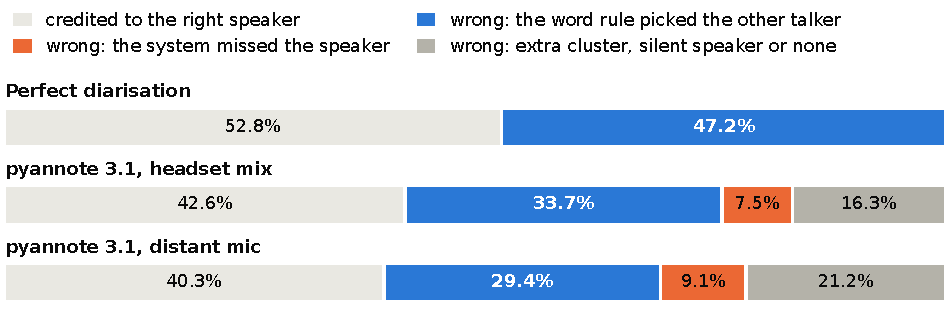
\includegraphics[width=\textwidth]{figures/fig2_word_outcomes.pdf}
\caption{\textbf{In overlap, the one-speaker-per-word rule misattributes more words than missed speakers do.} Outcome of each overlapped reference word of the AMI test set, with the true words and timings and no speech recognition; permutation-invariant mapping; 21,840 overlapped words, 16 meetings. Source: \texttt{results/attr\_oracle\_pyannote31/aggregate.csv}.}
\label{fig:outcomes}
\end{figure}

\textbf{The rule causes most of it.} When two speakers cover a word, the rule must pick one, and on AMI that choice is close to a coin flip; it sets a floor of about 12\% of all words before any diarisation error. For pyannote, the rule accounts for 34\% (headset) and 29\% (distant) of overlapped words, against 7.5\% and 9.1\% lost because the system missed the word's speaker. The tie-break does not decide this: crediting the speaker whose turn started first gives 52.1\% wrong with perfect diarisation, the one whose turn started last 38.6\%.

\textbf{Metric B is more lenient, not stricter.} It maps each system speaker to a person separately, so an extra cluster that splits one person costs nothing. Attribution error falls by 1.4 points [0.7, 2.2] on the headset mix and 2.4 [1.3, 3.5] on the distant microphone, and by 4.0 and 5.8 points in overlap. A one-to-one mapping fixed the same way gives exactly the permutation-invariant result, so all of the leniency comes from mapping several system speakers to one person: pyannote outputs 96 system speakers for the 63 people on the headset mix (4--9 per meeting) and 103 on the distant microphone.

\subsection{With speech recognition}\label{sec:asr}

With Whisper's words, pyannote's speaker-attributed WER is 33.4\% on the headset mix and 39.8\% on the distant microphone; most of it is transcription, and giving words to speakers costs more than diarisation (Table~\ref{tab:wer}, Figure~\ref{fig:parts}).

\begin{table}[htbp]
\centering
\caption{\textbf{Speaker-attributed WER over all words.}}
\label{tab:wer}
\small
\begin{tabular}{@{}lll@{}}
\toprule
 & Headset mix & Distant mic \\
\midrule
cpWER, perfect diarisation & 31.5\% [25.3, 37.0] & 36.3\% [29.9, 41.8] \\
cpWER, pyannote 3.1 & 33.4\% [26.7, 39.3] & 39.8\% [32.9, 46.0] \\
Fixed one-to-one mapping, pyannote 3.1 & 33.5\% & 39.8\% \\
Fixed many-to-one mapping (metric B), pyannote 3.1 & 31.4\% [25.4, 36.6] & 36.9\% [30.9, 42.1] \\
tcpWER (5~s collar), pyannote 3.1 & 34.5\% [27.6, 40.5] & 41.0\% [33.8, 47.3] \\
\bottomrule
\end{tabular}
\end{table}

\textbf{Whisper writes down one talker at a time.} Outside overlap it outputs 0.91 words per spoken word on the headset mix [0.89, 0.93]; in overlap, 0.46 [0.44, 0.49] (distant microphone: 0.86 and 0.43). With perfect diarisation, 56\% of overlapped words are deleted, and the most-deleted word there is ``yeah'' (11\% of those deletions). Overlap holds a quarter of the words and 61\% of the errors (53\% on the distant microphone).

\textbf{Three nested parts.} On the same Whisper words, I split cpWER into what remains when every output word may go to whichever person fits best (MeetEval's diarisation-invariant cpWER, so transcription only), what the one-speaker-per-word rule adds with perfect diarisation, and what pyannote's own errors add on top.

\begin{figure}[htbp]
\centering
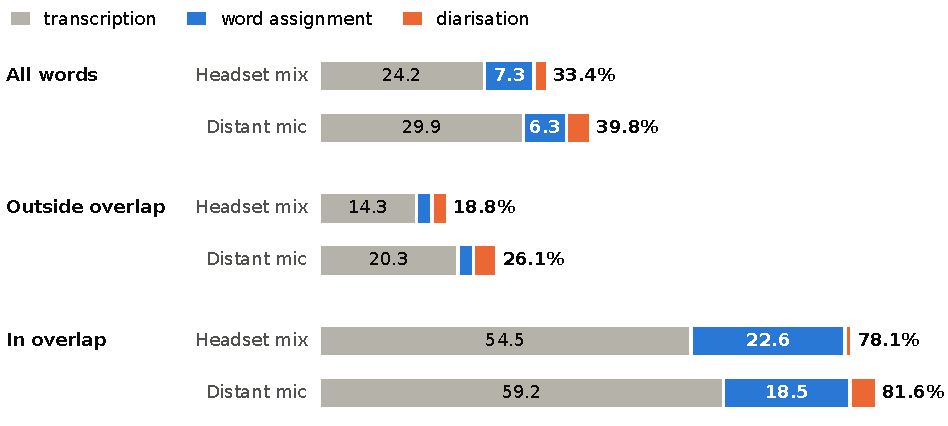
\includegraphics[width=\textwidth]{figures/fig3_cpwer_parts.pdf}
\caption{\textbf{Assigning words to speakers costs more word errors than diarisation does.} Speaker-attributed WER of pyannote 3.1 with Whisper (cpWER, \%), split into three nested parts: transcription is DI-cpWER (each word free to go to any person); the other two are what each later step adds. 89,443 reference words per microphone, 16 meetings. Source: \texttt{results/wer\_decomposition\_whisper\_turbo/aggregate.csv}.}
\label{fig:parts}
\end{figure}

On the headset mix the split is 24.2 + 7.3 + 2.0 points, and in overlap 54.5 + 22.6 + 1.0; the word rule costs more than diarisation in all 16 meetings. On the distant microphone, 39.8 = 29.9 + 6.3 + 3.5, with the word rule ahead in 13 of 16. tcpWER, the time-constrained score used to rank CHiME-8, is 1.1 to 1.2 points above cpWER, so the picture does not depend on that choice. How the last two parts split depends on which turns count as perfect diarisation (Section~\ref{sec:second}).

\textbf{The two fixed mappings separate two effects.} A one-to-one mapping fixed on single-speaker speech scores within 0.02 points of cpWER, so skipping the permutation search changes nothing. The many-to-one mapping of the plan scores 2.1 points lower on the headset mix [1.0, 3.2] and 2.9 on the distant microphone [1.6, 4.2], and 5.8 and 7.3 points lower in overlap, because it merges pyannote's extra clusters for free. In overlap on the headset mix it even scores pyannote (72.2\%) better than perfect diarisation (77.1\%).

\textbf{Checks.} My cpWER and DI-cpWER equal MeetEval's on every meeting and microphone. A first transcription run with Whisper's fallback decoding switched off looped on one meeting (``Uh.''\ 830 times over 27 minutes); I discarded it, reran with Whisper's default decoding, and now check every transcript for repeats. Both deviations from the plan were checked. Whisper large-v3 on two meetings gives 29.6\% cpWER with pyannote against turbo's 29.9\% (27.6\% for both with perfect diarisation). Re-timing every word with WhisperX's forced alignment changes the word-assignment part by $-0.1$ points [$-0.4$, 0.1], and in overlap from 22.6 to 22.9 points.

\subsection{Which overlapped words are lost}\label{sec:lost}

In overlap, Whisper keeps the louder talker and drops the quieter one, and pyannote tends to show the same talker. I measured each talker's level during each overlapped word from the individual headset channels, relative to the other talkers active at that moment (Figure~\ref{fig:level}).

\begin{figure}[htbp]
\centering
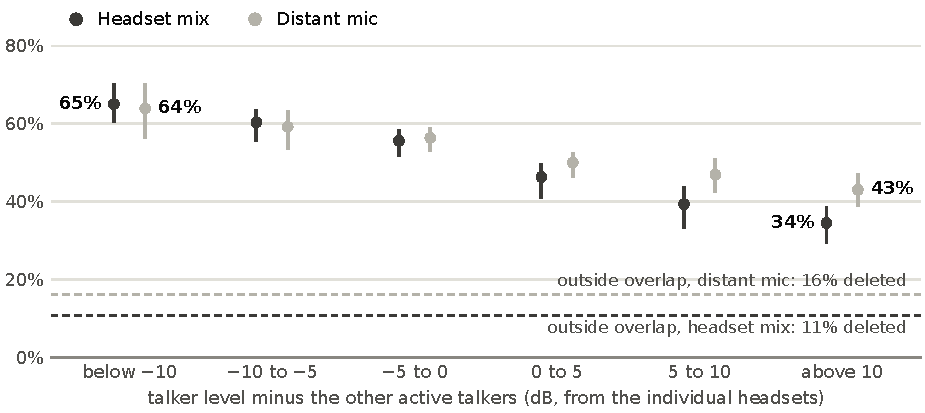
\includegraphics[width=\textwidth]{figures/fig4_deletion_by_level.pdf}
\caption{\textbf{In overlap, Whisper loses the quieter talker.} Share of overlapped words deleted by Whisper (transcription only), by the talker's level relative to the other active talkers; vertical bars are 95\% bootstrap intervals over the 16 meetings, dashed lines the deletion rate outside overlap. 22,105 overlapped reference tokens per microphone. Sources: \texttt{results/overlap\_words\_whisper\_turbo/aggregate.csv}; outside-overlap rates from \texttt{results/wer\_decomposition\_whisper\_turbo/aggregate.csv}.}
\label{fig:level}
\end{figure}

The effect is not a by-product of backchannels or turn order: it holds within turns of more than two words (64\% of words deleted below $-10$~dB, 32\% above +10~dB) and for the first and the second talker separately (59\% to 25\%, and 70\% to 42\%). On the distant microphone the trend is the same but shallower, 64\% to 43\%, in 14 of the 16 meetings. Headset crosstalk limits the measure: on words with a single talker it reads +21~dB (median), so levels above about +20~dB are not resolved.

\textbf{Interjections and late starters lose most.} Whisper drops 66\% [60, 71] of the words in turns of one or two words, three quarters of which are backchannels such as ``yeah'', ``okay'' and ``mm-hmm'', against 46\% in longer turns. It drops 54\% [51, 57] of the words of the talker who started second, against 40\% [34, 44] for the one holding the floor. The word rule shows the same asymmetry, giving 53\% of the second talker's overlapped words to the other person against 40\% of the first talker's, while its errors do not depend on level (44--49\% in every band).

\textbf{pyannote shows the louder talker too.} When it shows only one of two overlapping talkers, it is the louder one 71\% of the time [69, 73] on the headset mix and 66\% [62, 70] on the distant microphone. Diarisation and transcription therefore tend to fail on the same person.

\subsection{A second diariser and a second reference}\label{sec:second}

Which diariser has the lower DER depends on the reference's word timings, while the word-level scores do not flip; with Whisper's words, Sortformer's cpWER in overlap is 10.4 points below pyannote's.

The plan listed NeMo as an optional second system. I ran NVIDIA's streaming Sortformer v2.1~\cite{sortformer}, which outputs up to four speakers at once (AMI test meetings have three or four), unchanged on CPU. Sortformer is trained on AMI labels made by forced alignment, which have tighter word boundaries than the manual word times of the standard reference; Horiguchi et al.~\cite{horiguchi} publish those labels. I therefore scored both systems against both references: the same 16 meetings and words, only the timing differs. The forced-alignment labels have 22\% less speech and 44\% less overlapped speech (19.3\% of speaker time instead of 27.0\%).

\begin{figure}[htbp]
\centering
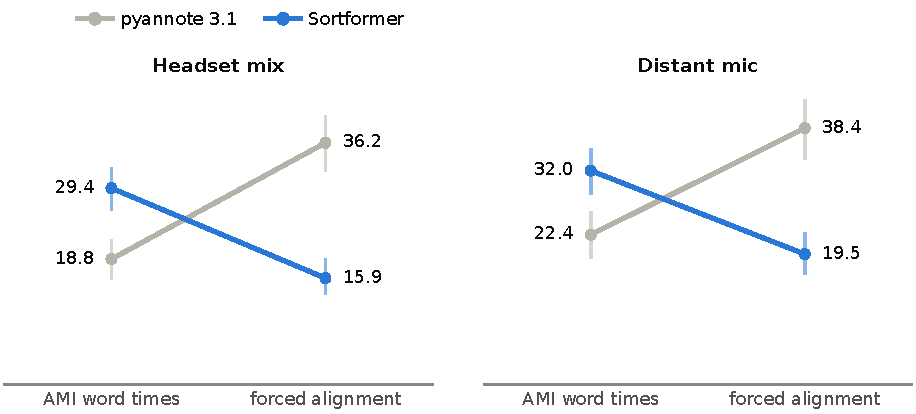
\includegraphics[width=\textwidth]{figures/fig5_reference_flip.pdf}
\caption{\textbf{Which system has the lower DER depends on the reference.} DER (\%, Full convention) of the same outputs against two references of the same 16 AMI test meetings: AMI's manual word times (the standard reference) and forced-alignment labels~\cite{horiguchi}. Vertical ticks are 95\% bootstrap intervals over meetings. Sources: \texttt{results/decomp\_sortformer\_v21/} and \texttt{results/decomp\_fa\_reference/} (\texttt{aggregate.csv}).}
\label{fig:flip}
\end{figure}

\textbf{The reference decides which system wins on DER} (Figure~\ref{fig:flip}). Against the standard reference, pyannote has the lower DER in all 16 meetings on both microphones; against the forced-alignment labels, Sortformer has it in 15 (headset mix) and 14 (distant microphone). pyannote marks the pauses inside AMI's word times as speech, which counts as false alarm against forced alignment (24.8\% of speaker time). Sortformer leaves them out, which counts as missed speech against the standard reference: it leaves unlabelled 52\% of the time inside reference words of 0.8~s or longer, against 11\% for pyannote.

\begin{table}[htbp]
\centering
\caption{\textbf{Word-level and overlap measures, standard reference.}}
\label{tab:systems}
\small
\begin{tabularx}{\textwidth}{@{}Lrrrr@{}}
\toprule
 & \multicolumn{2}{c}{Headset mix} & \multicolumn{2}{c}{Distant mic} \\
\cmidrule(lr){2-3}\cmidrule(l){4-5}
 & pyannote & Sortformer & pyannote & Sortformer \\
\midrule
cpWER with Whisper's words & 33.4\% & 32.7\% & 39.8\% & 39.7\% \\
cpWER in overlap & 78.1\% & 67.7\% & 81.6\% & 70.3\% \\
Speaker confusion in overlap & 13.9\% & 2.8\% & 16.1\% & 4.4\% \\
Overlapped true words credited to the wrong person & 57.4\% & 45.3\% & 59.7\% & 47.3\% \\
Shown talker is the louder, when one of two is shown & 71\% & 87\% & 66\% & 85\% \\
\bottomrule
\end{tabularx}
\end{table}

\textbf{Words give a stable comparison, and there Sortformer helps in overlap} (Table~\ref{tab:systems}). The two systems have the same cpWER over all words (paired difference $-0.8$ points [$-4.6$, 4.6] on the headset mix, $-0.05$ [$-4.3$, 5.2] on the distant microphone), but Sortformer's is 10.4 points lower in overlap [5.7, 13.5], in 14 of the 16 meetings (distant microphone: 11.3 points, in 13). It does not show more overlap than pyannote; it shows less (43\% of the overlapped time against 64\%). When it shows one of two talkers it is the louder one 87\% of the time, and Whisper keeps the louder talker, so the transcribed words usually go to the person who said them. The advantage holds when overlap is defined by the forced-alignment labels instead (7.0 points lower on the headset mix, 9.5 on the distant microphone); outside overlap, Sortformer's missed speech costs it 2 to 4 points.

\textbf{What changes in the earlier results.}
\begin{itemize}[leftmargin=*]
  \item For pyannote, overlap is three to five times harder per second under both references, but its share of the DER is not robust: against forced alignment, 19\% of pyannote's error is in overlap, its share of the time, because its false alarms in pauses dominate.
  \item The word rule's coin flip is robust: with forced-alignment turns as perfect diarisation, 43.3\% [41.9, 44.5] of overlapped words still go to the wrong person.
  \item The split of cpWER depends on which turns count as perfect diarisation. With forced-alignment turns, perfect diarisation gives 29.6\% instead of 31.5\% (67.9\% instead of 77.1\% in overlap). Word assignment then still costs more than diarisation on the headset mix (5.8 against 3.8 points), the two are about equal on the distant microphone (5.4 against 4.9), and pyannote's diarisation costs about 10 points in overlap rather than 1. Sortformer matches the forced-alignment turns in overlap (67.7\% against 67.9\%).
  \item For Sortformer, which cannot over-cluster, the many-to-one mapping of metric B forgives only 0.1 points [0.0, 0.4] on the headset mix, against 1.4 for pyannote, which confirms the over-clustering explanation.
\end{itemize}

Sortformer ran with its default post-processing. NVIDIA's published setting for this model family, tuned on DIHARD III, lowers its DER by 1.1--1.5 points and changes cpWER by less than 0.5. It handles at most four speakers, so I did not run it on the Supreme Court argument.

\subsection{The Supreme Court argument}\label{sec:scotus}

On a formal argument with long turns the same pipeline works well, and the fixed mapping is no longer lenient. I ran pyannote 3.1 and Whisper, unchanged, on the 62-minute argument in \emph{New York State Rifle \& Pistol Association v.\ City of New York} (2 December 2019, 10 speakers), against Oyez's turns and transcript (Table~\ref{tab:scotus}).

\begin{table}[htbp]
\centering
\caption{\textbf{Supreme Court argument, 62~min, 10 speakers.}}
\label{tab:scotus}
\small
\begin{tabularx}{\textwidth}{@{}Ll@{}}
\toprule
Measure & Value \\
\midrule
pyannote speakers found & 10, one per person (each 94--98\% one person) \\
DER, Full / Fair & 9.9\% / 8.3\% \\
\quad of which missed speech / false alarm / confusion (Full) & 7.4\% / 1.4\% / 1.1\% \\
Transcription only (DI-cpWER) & 5.1\% \\
cpWER with Oyez's turns (perfect diarisation) & 7.5\% \\
cpWER with pyannote 3.1 & 7.8\% \\
Fixed one-to-one and many-to-one mappings, pyannote 3.1 & 7.8\% (both equal cpWER) \\
\bottomrule
\end{tabularx}
\end{table}

With one cluster per person, all three mappings agree, which supports the explanation for AMI: the many-to-one mapping is lenient only where the system over-clusters. Most of the DER is missed speech because the Oyez reference marks all 62 minutes as speech, pauses included, while the system marks 59; this is why I use this set for attribution only. One recording gives no interval, so these numbers describe this case rather than courtroom speech in general.

\section{Discussion}

The results answer the plan's two questions and change what I would measure next.

\textbf{Metric B, as planned, hides errors instead of exposing them.} The fixed many-to-one mapping was meant to catch errors that permutation invariance hides. On these systems it forgives over-clustering instead, by 2.1 to 2.9 points of word error for pyannote, while a one-to-one mapping fixed the same way gives the permutation-invariant score. I would propose the fixed one-to-one version, with the number of extra clusters reported beside it, so that the measure stays strict and over-clustering is visible on its own.

\textbf{Most overlap errors are not diarisation errors.} In overlap, most of the word error is transcription: Whisper writes down one talker, and the quieter one is lost. Next comes the one-speaker-per-word rule, which misattributes 43--47\% of overlapped words even with perfect diarisation. Diarisation itself adds 1 point over the standard reference's turns and about 10 over forced-alignment turns. A better overlap detector alone cannot recover most of these words; recovering the quieter talker's audio, or deciding each word's speaker from acoustic evidence, can. Sortformer points the same way: it marks less overlap than pyannote but follows the talker who is actually audible, and gains 10 points of cpWER in overlap.

\textbf{DER comparisons need the reference's timing convention stated.} Two systems trained on references with different boundary conventions swap ranks on DER depending on the reference, while their word-level scores agree. For comparing systems on speaker-attributed transcription, word-level measures (cpWER and the attribution error) are the safer basis, and the DER decomposition is best reported against both references.

\section{Limitations and deviations from the plan}

Two deviations from the plan were forced by the CPU budget; both were checked and neither changes a finding.

\begin{itemize}[leftmargin=*]
  \item \textbf{Speech recognition model.} Whisper large-v3-turbo instead of large-v3. On two meetings, large-v3 gives the same cpWER within 0.4 points with pyannote; with $n = 2$ this bounds the effect rather than measuring it.
  \item \textbf{Word timing.} Whisper's own word times instead of WhisperX alignment. Re-timing all 16 headset-mix meetings with WhisperX changes each part of the decomposition by less than half a point over all words and by at most 1.2 points in overlap; 2 of 2,453 segments, both single words, could not be aligned and kept their times.
  \item \textbf{System outputs.} The pyannote numbers use the authors' published outputs; my own CPU run is a reproduction check, finished for 3 of 16 distant-microphone meetings so far.
  \item \textbf{Reference.} Main results use the standard only\_words reference, as planned; the forced-alignment labels serve as a check only.
  \item \textbf{Sortformer.} Default post-processing, at most four speakers, nothing tuned on AMI.
  \item \textbf{Level measure.} Headset crosstalk caps the measurable level at about +20~dB.
  \item \textbf{Sample size.} 16 meetings and 63 people, with intervals over meetings, so effects in small subgroups are uncertain; the Supreme Court result is one recording.
  \item \textbf{Text normalisation.} Normalising word by word does not join multi-word numbers (about 0.1\% of tokens); this affects every compared system equally.
\end{itemize}

\textbf{Corrections to my earlier emails.}
\begin{enumerate}[leftmargin=*, label=\arabic*.]
  \item \textbf{The 40.4-point result.} In my first email I said that relabelling one speaker moved that speaker's share of the generated notes by 40.4 points. Rechecking my earlier work, 40.4 points came from anonymising all speaker labels. A cyclic permutation of the labels, the case DER is invariant to, moved the share by only 3.6 points, below my 5-point threshold. The accurate claim is that the note generator uses speaker identity as structure, not that a label permutation changed the notes.
  \item \textbf{The Supreme Court ``gold'' set.} Its reference is built from Oyez's per-turn timings: 248 turns, 10 speakers, placed back to back with no overlap and no silence. It cannot support the overlap breakdown, and it cannot count speech in pauses as false alarm, so I use it for attribution only unless overlap is annotated.
\end{enumerate}

\section{Proposed next steps}

In this order, after your input on the questions below:

\begin{enumerate}[leftmargin=*, label=\arabic*.]
  \item \textbf{Recover the quieter talker before recognition.} Separate the talkers in overlapped regions, single-channel or by beamforming on AMI's array, and measure how much of the 54.5 + 22.6 points of overlap error it removes, against the level curve in Section~\ref{sec:lost}.
  \item \textbf{Overlap-aware word assignment.} Give each overlapped word to a speaker from acoustic evidence for that word (for example a speaker embedding of the word's audio) rather than from timestamps alone, to attack the word-assignment part directly.
  \item \textbf{Report against both references.} Run the DER decomposition and the attribution measures against the forced-alignment labels as well, unless you prefer one reference.
  \item \textbf{Close the remaining deviations.} Run Whisper large-v3 on the full test set once I have GPU time, and finish the CPU reproduction of pyannote 3.1.
\end{enumerate}

\section{Questions for you}

\begin{enumerate}[leftmargin=*, label=\arabic*.]
  \item Against forced-alignment labels of the AMI test set (Horiguchi et al.~\cite{horiguchi}), the DER ranking of pyannote and Sortformer flips, and the share of pyannote's error in overlap falls from 56\% to 19\%. Should I move the main results to those labels, or keep the standard reference and report the forced-alignment numbers as a check?
  \item Whisper loses the quieter talker in overlap, and both diarisers tend to show the louder one. Would you rather I first attack this acoustically, with separation or beamforming before recognition, or with an overlap-aware word assignment that leaves the audio as it is?
  \item The fixed mapping in the plan is many-to-one, so it forgives over-clustering, while a one-to-one fixed mapping gives the same score as cpWER here. Should metric B be one-to-one, with over-clustering reported as its own number, or is the many-to-one version what you intended?
  \item I ran NVIDIA's Sortformer as the optional second system. Would another overlap-aware system be more informative to you, such as NeMo's multi-scale model or one the group already uses?
  \item AMI's array channels are available to me. I would welcome pointers from you or Simon on recorded or simulated multichannel overlap, since spatial separation is one way to answer question 2.
\end{enumerate}

\begin{thebibliography}{10}
\small

\bibitem{ami}
\href{https://groups.inf.ed.ac.uk/ami/corpus/}{AMI Meeting Corpus}, University of Edinburgh; manual annotations 1.6.2, CC BY 4.0.

\bibitem{amisetup}
\href{https://github.com/pyannote/AMI-diarization-setup}{pyannote AMI diarization setup} (only\_words reference, full-corpus ASR partition).

\bibitem{pyannote}
\href{https://huggingface.co/pyannote/speaker-diarization-3.1}{pyannote/speaker-diarization-3.1} and \href{https://huggingface.co/pyannote/segmentation-3.0}{pyannote/segmentation-3.0}, model cards.

\bibitem{sortformer}
\href{https://huggingface.co/nvidia/diar_streaming_sortformer_4spk-v2.1}{NVIDIA streaming Sortformer 4spk v2.1}, model card; paper: \href{https://arxiv.org/abs/2507.18446}{Streaming Sortformer: speaker cache-based online speaker diarization with arrival-time ordering}, arXiv:2507.18446.

\bibitem{horiguchi}
S.~Horiguchi, N.~Tawara, T.~Ashihara, A.~Ando and M.~Delcroix, \href{https://arxiv.org/abs/2507.09226}{Can We Really Repurpose Multi-Speaker ASR Corpus for Speaker Diarization?}, IEEE ASRU 2025; \href{https://github.com/nttcslab-sp/diar-forced-alignment}{forced-alignment labels}.

\bibitem{meeteval}
T.~von Neumann, C.~Boeddeker, M.~Delcroix and R.~Haeb-Umbach, \href{https://arxiv.org/abs/2307.11394}{MeetEval: a toolkit for computation of word error rates for meeting transcription systems}, arXiv:2307.11394; \href{https://github.com/fgnt/meeteval}{toolkit}.

\bibitem{whisper}
A.~Radford et al., \href{https://arxiv.org/abs/2212.04356}{Robust speech recognition via large-scale weak supervision}, ICML 2023 (Whisper); \href{https://github.com/SYSTRAN/faster-whisper}{faster-whisper}.

\bibitem{whisperx}
M.~Bain, J.~Huh, T.~Han and A.~Zisserman, \href{https://arxiv.org/abs/2303.00747}{WhisperX: time-accurate speech transcription of long-form audio}, Interspeech 2023.

\bibitem{mdeval}
NIST md-eval-22.pl, as distributed with \href{https://github.com/nryant/dscore}{dscore}.

\bibitem{oyez}
\href{https://www.oyez.org/cases/2019/18-280}{Oyez: New York State Rifle \& Pistol Association v.\ City of New York}, argued 2 December 2019.

\end{thebibliography}

\appendix
\section{Reproducibility}

Every number here is computed from per-meeting result files, by scripts with one configuration file each, fixed seeds and a run log. \texttt{make all} re-scores the main steps from the committed system outputs; separate targets rerun diarisation, transcription and the further analyses. Each decision and deviation is logged with its reason in \texttt{docs/decisions.md}. The code, configurations and per-meeting results are in a repository I can share; audio is not included.

\begin{center}
\small
\begin{tabularx}{\textwidth}{@{}L>{\raggedright\arraybackslash}p{8.0cm}@{}}
\toprule
Analysis & Result directory \\
\midrule
Overlap-conditioned DER and overlap detection (Section~\ref{sec:der}) & \texttt{results/decomp\_pyannote31/}\newline \texttt{results/overlap\_detection\_pyannote31/} \\
Attribution with the true words (Section~\ref{sec:attr}) & \texttt{results/attr\_oracle\_pyannote31/} \\
Speaker-attributed WER, fixed mappings and its split (Section~\ref{sec:asr}) & \texttt{results/attr\_asr\_whisper\_turbo/}\newline \texttt{results/wer\_decomposition\_whisper\_turbo/} \\
Which overlapped words are lost (Section~\ref{sec:lost}) & \texttt{results/overlap\_words\_whisper\_turbo/}\newline \texttt{results/overlap\_dominance\_pyannote31/} \\
Sortformer against pyannote (Section~\ref{sec:second}) & \texttt{results/compare\_sortformer\_pyannote/}\newline \texttt{results/decomp\_sortformer\_v21/}\newline \texttt{results/wer\_decomposition\_sortformer\_v21/} \\
Forced-alignment reference (Section~\ref{sec:second}) & \texttt{results/decomp\_fa\_reference/}\newline \texttt{results/attr\_oracle\_fa\_reference/}\newline \texttt{results/wer\_decomposition\_fa\_regions/} \\
Supreme Court argument (Section~\ref{sec:scotus}) & \texttt{results/scotus\_pyannote31\_whisper/} \\
Per-meeting consistency of each claim & \texttt{results/consistency/}\newline \texttt{results/compare\_sortformer\_pyannote/} \\
Deviation and reproduction checks & \texttt{results/wer\_decomposition\_large\_v3\_subset/}\newline \texttt{results/wer\_decomposition\_wxalign/}\newline \texttt{results/reproduction\_pyannote31/} \\
Figures of this report & \texttt{report/make\_figures.py} \\
\bottomrule
\end{tabularx}
\end{center}

\end{document}
